Let $K$ be a knot and $D$ be its oriented diagram with $s$ segments and $x$ crossings. 
%The knot itself has the homotopy type of a circle and so its fundamental group is not interesting in itself. However, for a knot that is embedded in $S^3$ we can study the fun
\begin{definition}[knot group] 
  The fundamental group of a knot embedded in a three dimensional sphere $S^3$ is called a \buff{knot group}.
  $$\mathbf{\pi_1(K):=\pi_1(S^3-K)}.
  $$
\end{definition}
Although the knot itself is always a circle $S^1$, the knot group has usually an interesting yet difficult structure. The most known representation of the knot group is called \buff{the Wirtinger presentation}.

\begin{definition}[Wirtinger presentation]
  Given a diagram $D$ of knot $K$ with segments $a_1$, $a_2$, ..., $a_s$ and crossings $c_1$, ..., $c_x$ the knot group $\pi_1(K)$ can be represented as $\pi_1(K)=\langle G\;|\;R\rangle$, where $G$ is the set of segments of $D$ and relations $R$ correspond to crossings in the manner described in the diagram below
  \begin{center}
    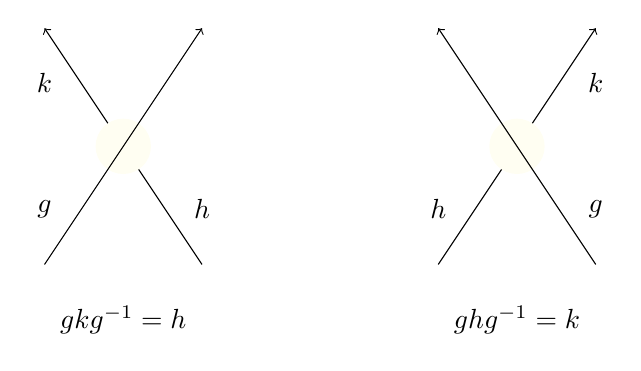
\begin{tikzpicture}
      \begin{scope}
        \draw[->] (2, 0)--(0, 3);
        \fill[yellow!5] (1, 1.5) circle (10pt);
        \draw[->] (0, 0)--(2, 3);
        \node at (0, .7) {$g$};
        \node at (0, 2.3) {$k$};
        \node at (2, .7) {$h$};

        \node at (1, -.7) {$gkg^{-1}=h$};
      \end{scope}

      \begin{scope}[shift={(5, 0)}]
        \draw[->] (0, 0)--(2, 3);
        \fill[yellow!5] (1, 1.5) circle (10pt);
        \draw[->] (2, 0)--(0, 3);
        \node at (0, .7) {$h$};
        \node at (2, 2.3) {$k$};
        \node at (2, .7) {$g$};
        
        \node at (1, -.7) {$ghg^{-1}=k$};
      \end{scope}
    \end{tikzpicture}
  \end{center}
  Representation $\langle G\;|\;R\rangle$ described above is called the \buff{Wirtinger presentation} \cite[Chapter~6]{livingstone}.
\end{definition}

An easily obtainable result, either by applying the Mayer-Vietoris sequence to $S^3=K\oplus S^3-K$ or noticing that every two generators are conjugate, is that the abelianization of the knot group is always $\Z$. This leads to an acyclic complex
\begin{center}
  \begin{tikzcd}
    0\arrow[r] & K_G \arrow[r] & G=\pi_1(K)\arrow[r, "ab"] & \Z=G^{ab} \arrow[r] & 0
  \end{tikzcd}
\end{center}

The group $K_G=\ker(ab:G\to\Z)=[G, G]$ is not finitely generated, an observation that is discussed in \cref{alexander module discussion}, and thus is a difficult group to work with. However, its abelianization $K_G^{ab}=K_G/[K_G, K_G]$ allows a $\Z[\Z]$ module structure and thus contains obtainable information about the knot $K$. 

The following is an exact sequence:
\begin{center}
  \begin{tikzcd}
    0\arrow[r] & K_G^{ab} \arrow[r] & G^{mab}=G/[K_G, K_G]\arrow[r] & \Z \arrow[r] & 0
  \end{tikzcd}
\end{center}
which gives foundation for the following definition.

% If $G$ is considered in its Wirtinger presentation, then $K_G$ does not have a finite set of generators. If $a_1$,..., $a_s$ where the generators of $G$ such that $(a_i)^{ab}=1$ for every $i$, then choosing new generators to be $x_i=a_ia_1^{-1}$ for $i=2,..., s$ implies that $K$ is generated by $a_1^{k}x_ia_1^{-k}$ for $i=2,...,s$ and $k\in\Z$.

\begin{definition}[metabelianization]\label{def:metabelianization}
  The quotient group $G^{mab}=G/[K_G, K_G]$ is called the \buff{metabelianization} of $G$. 
\end{definition}

We will return to the concept of metabelianization in \cref{section2}.




